%-*- japanese-latex -*-
%%% Local Variables:
%%% mode: japanese-latex
%%% TeX-master: "main"
%%% End:
% \underline{■■HERE■■}

%\renewcommand{\kanjifamilydefault}{\gtdefault}
\documentclass[a4paper,12pt]{jsarticle}
%\include{header}
\title{Rakefile for \LaTeX ~compile}
\author{Ippei KISHIDA}
\date{Last-modified: 2017/05/09 12:45:55.}

\usepackage{graphicx,float,textcomp,ascmac,amsmath,amssymb,color}

\newcommand{\eqlabel}[1]{\label{#1} \hspace{10mm} (\mathrm{#1})} %equation label with displaying label
\newcommand{\eqrefInEq}[1]{\notag \hspace{10mm} \mathrm{\#\eqref{#1}}} %equation reference in Equation
\newcommand{\n}{\notag \\} %newline in equation without tag
\newcommand{\chem}[1]{$\mathrm{#1}$ } %chemical equation
\newcommand{\itemLabel}[1]{\item (#1) \label{#1}}

\newtoks\tmpId %temporary ID for figure and table

% in preamble
\usepackage{listings}
\lstset{%
  language={Ruby},
  %backgroundcolor={\color[gray]{.90}},%
  backgroundcolor={\color[rgb]{1.0,0.95,0.95}},%
  %basicstyle={\footnotesize},%
  %identifierstyle={\footnotesize},%
  %commentstyle={\footnotesize\itshape},%
  %keywordstyle={\footnotesize\bfseries},%
  %ndkeywordstyle={\footnotesize},%
  %stringstyle={\footnotesize\ttfamily},
  frame={tb},
  breaklines=true, % 長すぎる行の途中で自動的に改行
  %columns=[l]{fullflexible},%
  numbers=left,%
  xrightmargin=0zw,%
  xleftmargin=1zw,%
  %numberstyle={\scriptsize},%
  %stepnumber=1,
  %numbersep=0.5zw,%
  lineskip=-0.5ex%
}
\renewcommand{\lstlistingname}{List}


\begin{document} %----------------------------------------------------
\maketitle
\tableofcontents


\section{生成の流れと依存関係}
\label{sec010}

(English version will be written in \S\ref{sec020}.)

Fig.~\ref{fig010} に生成の流れを示す。
tex ファイルから dvi を生成し、dvi から pdf を生成を生成するというのがメインのプロセス。
dvi を生成する際に eps が必要になる。
eps は graphviz 系、 gnuplot、 ruby など様々な方法で生成される。
\LaTeX は印刷を最終目的とするものなので、
ベクターデータである eps での出力が主となる。
とはいえ eps だと閲覧が不便で、qiv などで簡便に表示するために png があったら便利。
ということで \LaTeX で扱う画像は、
ベクターデータ( eps )が主であり、
ラスターデータ( png )が補助的という位置付けとなる。
\footnote{
  この点が Markdown/HTML と決定的に異なる。
  Markdown/HTML はディスプレイで表示するのを目的とするため
  ラスターデータ( png )が主であり、
  ベクターデータ( eps )が補助的という位置付けになる。
}

\begin{figure}[!htbp]
  \tmpId={fig010}
  \begin{center}
    \includegraphics[width=1.0\linewidth]{\the\tmpId.eps} %
    %\includegraphics{\the\tmpId.eps} %
  \end{center}
  \caption{(\the\tmpId)
    \label{\the\tmpId}
    Generation flow from TEX to PDF.
    Each TEX file, *.tex, may become a top level TEX file and an included TEX document.
    Ruby script file, *.rb,
    may be embedding code in a list environment,
    and may be a gnuplot script for drawing a graph.
    Data file, *.dat, is assumed to be used as a data file in ruby and gnuplot.
    The flow necessary to make pdf is black, the process to make png which is supplementary treatments is red.
  }
\end{figure}

\paragraph{tex の問題}

本来の \LaTeX では、
ディレクトリ内のあらゆる tex ファイルが dvi を生成する可能性がある。
ファイルの中身を見て include 解析などすれば機械的に依存関係を把握できる筈だが、
ファイル名のみからはその関係がわからない。
しかも C のようにとりあえず単体が完結して
コンパイルできるということは保証されておらず、
documentclass 宣言や document 環境が
含まれていなければコンパイルできない。
ファイル名のみから判断される機械的なコンパイル動作を作るのは煩雑。
ソースコード解析してまでやるべきことではなかろう。

これらを解決するために自分ルールを導入する。
1つのディレクトリは 1つの pdf ファイルを生成するためのものと位置付ける。
latex で処理するのは唯一 main.tex のみとする。
ただし他の \verb/*.tex/ ファイルも依存する可能性があり更新時刻チェックの対象とする。
同じディレクトリにあるのだから include などで取り込まれるのだろう、
ということを前提とする。

\paragraph{pdf の名前}

「latex で処理するのは唯一 main.tex のみとする」ため、
素直に作ると main.dvi から main.pdf を生成することになる筈だが、
pdf を別の場所に移したりメール添付する場合には内容を表すファイル名に
その都度変更すべきという事になる。

自分ルールとして
「1つのディレクトリは 1つの pdf ファイルを生成するためのものと位置付ける」
ことから、カレントディレクトリの名前を用いたファイル名で PDF を作ることにする。
カレントディレクトリが foo ならば、foo.pdf である。

\paragraph{pov の問題}

pov の出力が png であり、eps には png を経由して生成するものであるということが問題。
そのため、svg などでは eps から png を生成するが、
pov では png から eps を生成することになり、
ファイルタイプ(拡張子)だけからはどちらがどちらに依存しているか
判別がつかないことになる。
rake を実行するたびに相互に生成しあうこともありうる。

これを解決するために、
rake の処理としては pov → eps に直接変換するように見えるようにする。
すなわち、内部的には png を生成するものの中間ファイルを削除する。

\paragraph{rb の問題}

rb ファイルが本当に画像を生成させるためのものかも問題。
プログラミングの教科書だと LIST 環境で表示するための
コードを記述していることもありうる。

この解決として、以下の自分ルールを課すことにする。

\begin{itemize}
  \item 画像用の rb ファイルは fig から始まるファイル名にする。
  \item LIST 環境で使うものは list から始まるファイル名にする。
  \item これら以外の rb ファイルは無視する。
\end{itemize}



\paragraph{dot の問題}

dot は graphviz の dot 形式ファイル。
ただし、 dot, circo, fdp, neato, twopi のいずれを使うかで描画され方が違う。
絵の意図としてはその都度どれかを選択する筈だが、
ファイル内でそれを指定できない。
(dot ファイルは基本的に論理的な関係のみを記述する。)
よって、ファイルごとに Rakefile に記述していく手間が生じることになる。

この解決として、
circo, fdp といった拡張子だったら
それらのコマンドを使うというルールを自分ルールとして採用。


\subsection*{自分ルールを含めて改善した生成の流れ}

上記の自分ルールの適用によって整理した生成の流れを Fig.~\ref{fig015} に示す。
このフローに沿って Rakefile を作成した。

\begin{figure}[!htbp]
  \tmpId={fig015}
  \begin{center}
    \includegraphics[width=1.0\linewidth]{\the\tmpId.eps} %
    %\includegraphics{\the\tmpId.eps} %
  \end{center}
  \caption{(\the\tmpId)
    \label{\the\tmpId}
    Improved generation flow including my own rules.
    Red arrows indicates processes to make PNG files. 
  }
\end{figure}

\section{Compiling process and dependency(English Version of \S \ref{sec010})}

\label{sec020}

The flow of generation is shown in Fig.~\ref{fig010}.
The main process is to generate DVI from the TEX file and generate pdf from DVI.
You need EPS files when generating DVI using figures.
EPS files are generated by various methods such as graphviz, gnuplot, and ruby.
The final objective of \LaTeX is printing.
Principal figure format should be EPS as vector data.
However, PNG is more convenient to display and browse than EPS.
\footnote{
  This point is definitely different from Markdown/HTML system.
  Markdown/HTML is intended to show on the electronic display.
  Raster data (PNG) is the main, Vector data (EPS) is not needed.
}



\paragraph {TEX problem}

In the original \LaTeX,
every TEX file in a directory may generate DVI.
Although you can grasp dependency mechanically by reading and analyzing the contents of the file,
it cannot be determined from the file name alone.
Moreover, not all tex file can be compiled unlike C.
Documentclass declaration and document environment must be included in
an entry point TEX file.
It is cumbersome to make a mechanical compilation operation judged
only from the file name.
It should not be done until analyzing the source code because of the complication.

I introduce my own rules to solve these problems.
One directory is positioned to generate one PDF file.
Only \verb/main.tex/ is compiled by latex.
However, other \verb/*.tex/ files may depend on them,
and they are used for the update time check.
It is based on the premise that
it will be included because they are in the same directory, 

\paragraph {PDF name}

"Only \verb/main.tex/ is compiled by latex."
Under the rule,
\verb/main.tex/ will generate \verb/main.dvi/ and \verb/main.pdf/.
But when the PDF is transferred to another place or attaching e-mails,
it should be renamed each time.
As my rule
"Position one directory as one for generating one pdf file".
Therefore, we will make a PDF with the file name using the name of the current directory.
If the current directory is \verb|foo/|, it is \verb/foo.pdf/ in the \verb|foo/| directory.

\paragraph {POV problem}

Many program can output EPS and PDF.
But POV-Ray can generate PNG but cannot EPS.
So EPS of POV-Ray figures are generated from PNG.
It is a problem that
it is difficult to determine the first of EPS and PNG from mechanically.

In order to solve this problem,
a process is imitated like to make EPS directly from POV.
That is, internally, it creates png but deletes the intermediate file.

\paragraph {RB problem}

It is also a problem whether the RB file is really for generating images.
The ruby code may be LIST environment material for programming textbooks.
To solve this, we will impose our own rule.


\begin{itemize}
  \item The RB file for images should be filenames starting with \verb/fig/, e.g., \verb/fig010.rb/.                 
  \item The one used in the LIST environment is the file name starting from the \verb/list/, e.g., \verb/list010.rb/. 
  \item Ignore other RB files.                                                  
\end{itemize}


\paragraph {DOT problem}

DOT is a file for graphviz.
However, the figure is generated by various commands, e.g., dot, circo, fdp, neato, twopi, etc.
%The dot file should include only the logical relation.
As the intention of the picture, you should choose something every time,
it can not be specified in the file.
Therefore, it takes time and effort to describe it in the Rakefile for each file.

As this solution,
I assume new extensions like \verb/.circo, .fdp/, etc.
We adopt the rule of using those commands as our rule.

\subsection*{Improved generation flow including my own rules}

The flow of generation sorted out by applying the above rule of self is shown in Fig.~\ref{fig015}.
I made a Rakefile along this flow.


\section{Misc}

\subsection{Requirement}

\begin{itemize}
  \item latex
  \item latexmk
  \item bibtex
  \item dvipdfmx
  \item gnuplot
  \item graphviz
  \item imagemagick
  \item inkscape
  \item povray
  \item (ruby/gnuplot)
\end{itemize}

\subsection{License}

MIT license.

\subsection{Usage}

\begin{verbatim}
rake dvi
rake pdf
rake png
rake clean
\end{verbatim}


\section{Section for test}

\subsection{Other *.tex}

「この文は input1.tex 内に記述されている。」

"This sentense is written in input1.tex"




\subsection{list}

\tmpId={list010.rb}
\lstinputlisting[caption=(\the\tmpId)list010.rb]{\the\tmpId}


\subsection{Figures}

Conversion from 'dot' to 'eps' can be confirmed at Fig. \ref{fig010}.

\begin{figure}[!htbp]
  %\tmpId={fig020}
  \begin{center}
  %\includegraphics[width=1.0\linewidth]{\the\tmpId.eps} %[width=1.0\linewidth]
  \includegraphics[width=0.3\linewidth]{fig020.eps} %[width=1.0\linewidth]
  \includegraphics[width=0.3\linewidth]{fig030.eps} %[width=1.0\linewidth]
  \includegraphics[width=0.3\linewidth]{fig040.eps} %[width=1.0\linewidth]
  \end{center}
  \caption{(\the\tmpId)
    \label{fig020_030_040}
    circo (fig020),
    fdp (fig030),
    neato (fig040),
  }
\end{figure}


\begin{figure}[!htbp]
  \begin{center}
  \includegraphics[width=0.3\linewidth]{fig070.eps} %[width=1.0\linewidth]
  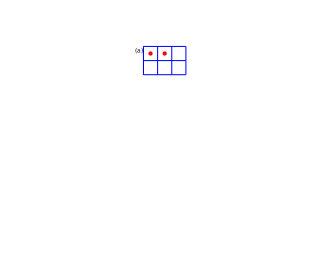
\includegraphics[width=0.3\linewidth]{fig080.eps} %[width=1.0\linewidth]
  %\includegraphics{\the\tmpId.eps} %[width=1.0\linewidth]
  \end{center}
  \caption{
    \label{fig070_080}
    pov → eps (fig070),
    svg → eps (fig080)。
  }
\end{figure}

\begin{figure}[!htbp]
  %\tmpId={fig090}
  %\tmpId={fig100}
  \begin{center}
  \includegraphics[width=0.4\linewidth]{fig090.eps} %[width=1.0\linewidth]
  \includegraphics[width=0.4\linewidth]{fig100.eps} %[width=1.0\linewidth]
  \end{center}
  \caption{(\the\tmpId)
    \label{fig090_100}
    rb + dat → eps (fig090),
    plt + dat → eps (fig100).
  }
\end{figure}


\end{document}

